%\documentclass[12pt,fullpage,doublespace]{elsart}
\documentclass[10pt,twocolumn]{elsart5p}
\usepackage{graphicx}
\usepackage{dcolumn}
\usepackage{amsmath}
\usepackage{amssymb}
\usepackage{bm}
\usepackage{natbib}

% 
%
% Introduction
% ============
%
% Measures
% ========
% ISI
% SPIKE
% Edge effect
% SPIKE-realtime
% SPIKE-future
% Representations
% Spike train surrogates (Significance), Comparison with Poisson
% Computational Cost (Memory, Speed)
%
% SPIKY
% =====
% Input (data format), Spike Train Generator (Patterns, by hand) 
% Output
% Figure Layout
% GUI vs Loop
% Comparison with other measures/implementations
%
% Discussion
% ==========
% Limitations
% Outlook
%
%
%



\begin{document}

\begin{frontmatter}

\title{SPIKY: A graphical user interface for monitoring spike train synchrony}

\author{Nebojsa Bozanic},
\ead{strance@gmail.com}
\author{Thomas Kreuz}
\ead{thomas.kreuz@cnr.it}


\address{Institute for complex systems, CNR, Sesto Fiorentino, Italy}


\date{\today}

\begin{abstract}
    Recently, the SPIKE-distance has been proposed as a measure of spike train synchrony which is both parameter-free and time-scale independent. Since it relies on instantaneous estimates of spike train dissimilarity, it is also time-resolved which makes it possible to track changes in instantaneous clustering, i.e., time-localized patterns of (dis)similarity among multiple spike trains. Further features include selective and triggered temporal averaging as well as the instantaneous comparison of spike train groups. Besides the regular SPIKE-distance, there also exists a causal variant which is defined such that the instantaneous values of dissimilarity rely on past information only so that time-resolved spike train synchrony can be estimated in real-time. Finally, here we introduce the future SPIKE-distance which can be used in triggered temporal averaging in order to evaluate the effect of certain spikes or of certain stimuli features on future spiking. In the first part of this report we address some of the computational aspects in the calculation and implementation of the SPIKE-distance while in the second part we present SPIKY, a graphical user interface which facilitates the application of the SPIKE-distance and all its variants to both simulated and real data.
\end{abstract}


%\begin{keyword}
%    time series analysis; spike trains; clustering; neuronal coding
%\end{keyword}

\end{frontmatter}

\newcommand{\abb}{\small\sf}

%
% ********************************************************************************************** Intro **************
%
\section{\label{s:Intro} Introduction}

A wide variety of approaches to quantify the dissimilarity, or distance, between two spike trains has been suggested. Among these is the metric introduced in \citet{Victor96}, which evaluates the cost needed to transform one spike train into the other, using only certain elementary steps. Another metric proposed in \citet{VanRossum01}, measures the Euclidean distance between the two spike trains after convolution of the spikes with an exponential function. Both methods involve one parameter that sets the time scale. In contrast, two more recent bivariate approaches, the ISI- and the SPIKE-distance are time scale independent and self-adaptive \citep{Kreuz07c, Kreuz13}. These two measures are complementary: The ISI-distance relies on the relative length of simultaneous interspike intervals and is thus well-designed to quantify similarities in the neurons� firing-rate profiles \citep{Kreuz07c, Kreuz09}. The SPIKE-distance is based on differences between the spike times of the two spike trains and is therefore ideally suited to track synchrony that is mediated by spike timing \citep{Kreuz11, Kreuz13}.

XXXXX Computational aspects XXXXX

%
% **************************************************************** Methods **************
%
\section{\label{s:Measures} Measures}

% XXXXX maybe shift definition of distances to the appendix XXXXX



\subsection{\label{ss:SPIKE-Distance} The SPIKE-distance}

The SPIKE-distance (see \citet{Kreuz11} for the original proposal and \citet{Kreuz13} for the definite version presented here) is extracted from differences between the spike times of the two spike trains. It relies on instantaneous values in the sense that in a first step the two sequences of discrete spike times are transformed into a continuous dissimilarity profiles $S (t)$. This dissimilarity profile is based on three piecewise constant quantities which for each neuron $n = 1, 2$ are assigned to every time instant between $0$ and $T$ (see Fig. \ref{fig:Fig1-SPIKE-Illustration}). These are the time of the preceding spike
%
\begin{equation} \label{eq:Prev-Spike}
    t_{\mathrm {P}}^n (t) = \max(t_i^n | t_i^n \leq t)  \quad t_1^n \leq t \leq t_{M_n}^n,
\end{equation}
%
the time of the following spike
%
\begin{equation} \label{eq:Foll-Spike}
    t_{\mathrm {F}}^n (t) = \min(t_i^n | t_i^n > t)  \quad t_1^n \leq t \leq t_{M_n}^n,
\end{equation}
%
as well as the interspike interval
%
\begin{equation} \label{eq:ISI}
    x_{\mathrm {ISI}}^n (t) = t_{\mathrm {F}}^n (t) - t_{\mathrm {P}}^n (t).
\end{equation}
%
The ambiguity regarding the definition of the very first and the very last interspike interval is resolved by placing for each spike train auxiliary leading spikes at time $t = 0$ and auxiliary trailing spikes at time $t = T$.
%
\begin{figure}
    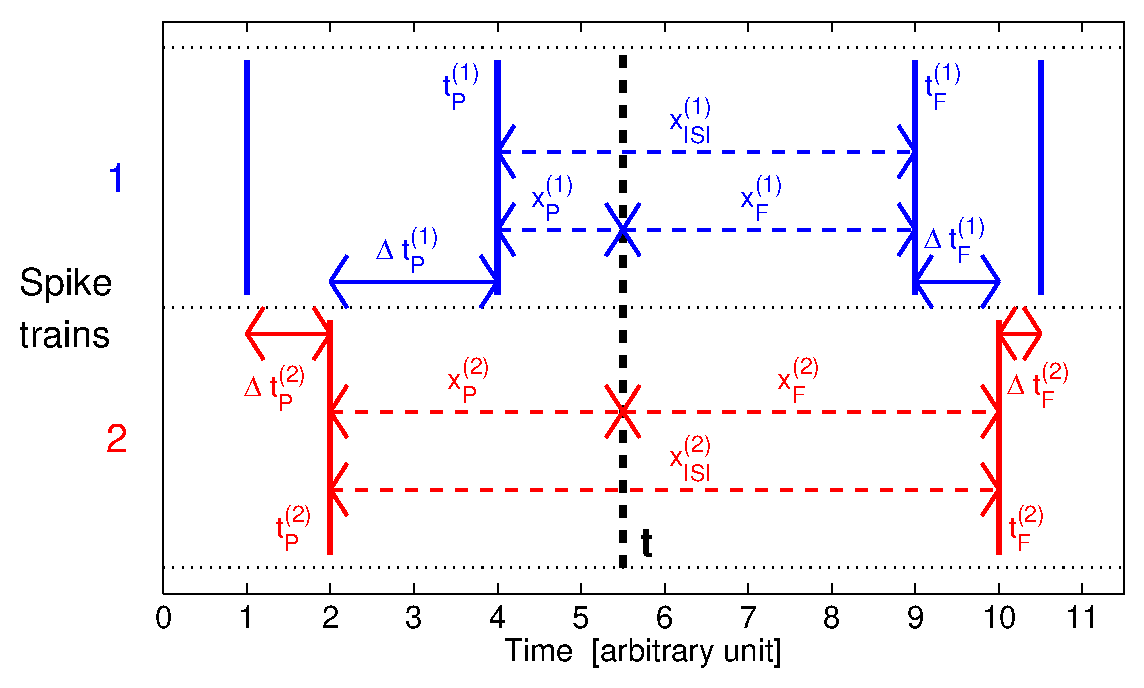
\includegraphics[width=85mm]{Fig1_SPIKE_Illustration.eps}
    \caption{\abb\label{fig:Fig1-SPIKE-Illustration} SPIKE-distance. Illustration of the local quantities needed to define the dissimilarity profile $S (t)$ for an arbitrary time instant $t$.}
\end{figure}
%
From these three quantities the dissimilarity profile is calculated in two steps: First for each spike the distance to the nearest spike in the other spike train is calculated, then for each time instant the relevant spike time differences are selected, weighted, and normalized. Here �relevant� means local; each time instant is uniquely surrounded by four corner spikes: the preceding spike from the first spike train $t_{\mathrm {P}}^{(1)}$, the following spike from the first spike train $t_{\mathrm {F}}^{(1)}$, the preceding spike from the second spike train $t_{\mathrm {P}}^{(2)}$, and, finally, the following spike from the second spike train $t_{\mathrm {F}}^{(2)}$. Each of these corner spikes can be identified with a spike time difference, for example, for the previous spike of the first spike train
%
\begin{equation} \label{eq:Delta-Corner-Spike}
     \Delta t_{\mathrm {P}}^{(1)} = \min_i (| t_{\mathrm {P}}^{(1)} - t_i^{(2)} |)
\end{equation}
%
and analogously for $t_{\mathrm {F}}^{(1)}$, $t_{\mathrm {P}}^{(2)}$, and $t_{\mathrm {F}}^{(2)}$  (see Fig. \ref{fig:Fig1-SPIKE-Illustration}). For each spike train separately a locally weighted average is employed such that the differences for the closer spike dominate; the weighting factors depend on
%
\begin{equation} \label{eq:Prev-Spike-Dist}
     x_{\mathrm {P}}^{(n)} (t) = t - t_{\mathrm {P}}^{(n)} (t)
\end{equation}
%
and
%
\begin{equation} \label{eq:Foll-Spike-Dist}
     x_{\mathrm {F}}^{(n)} (t) = t_{\mathrm {F}}^{(n)} (t) - t,
\end{equation}
%
the intervals to the previous and the following spikes for each neuron $n = 1, 2$. The local weighting for the spike time differences of the first spike train reads
%
\begin{equation} \label{eq:Bi-Spike-Diss-Improved-First}
     S_1 (t) = \frac{\Delta t_{\mathrm {P}}^{(1)} x_{\mathrm {F}}^{(1)} + \Delta t_{\mathrm {F}}^{(1)} x_{\mathrm {P}}^{(1)}}{x_{\mathrm {ISI}}^{(1)}}
\end{equation}
%
and analogously $S_2 (t)$ is obtained for the second spike train. Averaging over the two spike train contributions and normalizing by the mean interspike interval yields
%
\begin{equation} \label{eq:Bi-Spike-Diss-Improved-Intermediate}
     S'' (t) = \frac{S_1 (t) + S_2 (t)}{2 \langle x_{\mathrm {ISI}}^{(n)} \rangle_n}.
\end{equation}

This quantity weights the spike time differences for each spike train according to the relative distance of the corner spike from the time instant under investigation. This way relative distances within each spike train are taken care of, while relative distances between spike trains are not. In order to get these ratios straight and to account for differences in firing rate, in a last step the two contributions from the two spike trains are locally weighted by their instantaneous interspike intervals. This leads to the improved definition of the dissimilarity profile
%
\begin{equation} \label{eq:Bi-Spike-Diss-Improved}
     S (t) = \frac{S_1 (t) x_{\mathrm {ISI}}^{(2)} + S_2 (t) x_{\mathrm {ISI}}^{(1)}}{2 \langle x_{\mathrm {ISI}}^{(n)} \rangle_n^2}.
\end{equation}

The SPIKE-distance is defined as the temporal average of this dissimilarity profile
%
\begin{equation} \label{eq:Temporal-Average}
    D_S = \frac{1}{T} \int_{0}^T dt S (t).
\end{equation}
%
The dissimilarity profile $S (t)$ and the SPIKE-distance $D_S$ as its average are bounded in the interval $[0, 1]$. The distance value $D_S = 0$ is obtained for identical spike trains only.

There exists a straightforward extension to the case of more than two spike trains (number of spike trains $N > 2$), the averaged bivariate distance. This average over all pairs of neurons commutes with the average over time, so it is possible to achieve the same kind of time-resolved visualization as in the bivariate case by first calculating the instantaneous average, e.g., $S^{\mathrm {a}} (t)$ over all pairwise instantaneous values $S^{mn} (t)$,
%
\begin{equation} \label{eq:Bivariate-Average}
    S^{\mathrm {a}} (t) = \frac{1}{N(N-1)/2}\sum_{n=1}^{N-1} \sum_{m=n+1}^N S^{mn} (t)
\end{equation}




xxx We define the ISI as going from right after the last spike to the exact time of the next spike. So the previous spike is not part of the ISI while the following is. So when you are on a spike this is the following spike and the one before is the previous spike. xxx not needed anymore xxx


\subsubsection{\label{sss:Edge-effect} Edge effect}

Conor's Email:

My instinct is to count the edge spikes as normal spikes, that is work out their gaps in the normal way but in the time before the first spike use the first spike as both the previous and next gap, similarly for the time after the last spike. This is different to having the extra spikes, that means taking the first and last real gap at half weight. The difficulty is with the ISI. We know two things about the ISI. Taking the example of the first spike, say it is at $t_1$ and the interval starts at $t=0$. Firstly the ISI shouldn't be smaller than $t_1$ and secondly, we know the ISI $t_2-t_1$ where $t_2$ is the time of the second spike. The thing is that if $t_1 < t_2-t_1$ it could be because $t_1 < "the true ISI"$, so one possibility is to take $max(t_1,t_2-t_1)$.

(Conor Houghton, personal communication)


\subsection{\label{ss:Realtime-Spike-Distance} Realtime SPIKE-distance}

The realtime SPIKE-distance $D_{S_r}$ is a modification of the SPIKE-distance with the key difference that the corresponding time profile $S_r(t)$ can be calculated online because it relies on past information only. From the perspective of an online measure, the information provided by the following spikes, both their position and the length of the interspike interval, is not yet available. Like the regular (improved) SPIKE-distance $D_S$, this causal variant is also based on local spike time differences but now only two corner spikes are available, and the spikes of comparison are restricted to past spikes, e.g., for the preceding spike of the first spike train
%
\begin{equation} \label{eq:Delta-Corner-Spike-Realtime}
     \Delta t_{\mathrm {P}}^{(1)} = \min_i (| t_{\mathrm {P}}^{(1)} - t_i^{(2)} |), t_i < t.
\end{equation}
%
Since there are no following spikes available, there is no local weighting, and since there is no interspike interval, the normalization is achieved by dividing the average corner spike difference by twice the average time interval to the preceding spikes (Eq. \ref{eq:Prev-Spike-Dist}). This yields a causal indicator of local spike train dissimilarity:
%
\begin{equation} \label{eq:Bi-Spike-Diss-RT}
    S_r (t) = \frac{ \Delta t_{\mathrm {P}}^{(1)} + \Delta t_{\mathrm {P}}^{(2)}} {4 \langle x_{\mathrm {P}}^{(n)} \rangle_n}.
\end{equation}


\subsection{\label{ss:Future-Spike-Distance} Future SPIKE-distance}

The future SPIKE-distance $D_{S_f}$ can be used in triggered temporal averaging in order to evaluate the effect of certain spikes or of certain stimuli features on future spiking. It is the inverse measure to the Realtime SPIKE-distance but instead of relying on past information only it relies on future information only. Also in this case for each time instant just two corner spikes are available, since the spikes of comparison are restricted to future spikes only. Thus the spike time difference for the following spike of the first spike train reads
%
\begin{equation} \label{eq:Delta-Corner-Spike-Future}
     \Delta t_{\mathrm {F}}^{(1)} = \min_i (| t_{\mathrm {F}}^{(1)} - t_i^{(2)} |), t_i > t,
\end{equation}
%
and accordingly for the following spike of the second spike train. And, similar to Eq. \ref{eq:Bi-Spike-Diss-RT}, an indicator of local spike train dissimilarity is obtained as follows:
%
\begin{equation} \label{eq:Bi-Spike-Diss-FT}
    S_f (t) = \frac{ \Delta t_{\mathrm {F}}^{(1)} + \Delta t_{\mathrm {F}}^{(2)}} {4 \langle x_{\mathrm {F}}^{(n)} \rangle_n}.
\end{equation}




\subsection{\label{ss:ISI-Distance} The ISI-distance}

While the dissimilarity profile of the SPIKE-distance is extracted from differences between the spike times of the two spike trains, the dissimilarity profile of the ISI-distance \citep{Kreuz07c, Kreuz09} is calculated as the instantaneous ratio between the interspike intervals $x_{\mathrm {ISI}}^{(1)}$ and $x_{\mathrm {ISI}}^{(2)}$ (Eq. \ref{eq:ISI}) according to:
%
\begin{equation} \label{eq:ISI-Ratio}
    I (t) = \begin{cases}
           x_{\mathrm {ISI}}^{(1)} (t) / x_{\mathrm {ISI}}^{(2)} (t) - 1 & {\rm if} ~~ x_{\mathrm {ISI}}^{(1)} (t) \leq x_{\mathrm {ISI}}^{(2)} (t) \cr
                      - (x_{\mathrm {ISI}}^{(2)} (t) / x_{\mathrm {ISI}}^{(1)} (t) -1)     & {\rm otherwise}.
                  \end{cases}
\end{equation}
%
This ISI-ratio equals $0$ for identical ISI in the two spike trains, and approaches $-1$ and $1$, respectively, if the first or the second spike train is much faster than the other. For the ISI-distance the temporal averaging analogous to Eq. \ref{eq:Temporal-Average} 
is performed on the absolute value of the ISI-ratio, thus both kinds of deviations are treated equally. Since the ISI-distance relies on the instantaneous ISI-values and thus requires knowledge about the following spikes, no causal Realtime extension is possible.


\subsection{\label{ss:Representations} Representations}

The ISI- and the SPIKE-distance combine a variety of properties that make them well suited for applications to real data. In particular, they are conceptually simple, computationally efficient, and easy to visualize in a time-resolved manner. By taking into account only the preceding and the following spike in each spike train, these distances rely on local information only. They are also time-scale-adaptive since the information used is not contained within a window of fixed size but rather within a time frame whose size depends on the local rate of each spike train.

Moreover, the sensitivity to spike timing and the instantaneous reliability achieved by the SPIKE-distance opens up many new possibilities in multi-neuron spike train analysis \citep{Kreuz13}. These build upon the fact that there are several levels of information reduction.

\subsubsection{\label{sss:Full-matrix-and-cross-sections} Full matrix and cross sections}

The starting point is the most detailed representation in which one instantaneous value is obtained for each pair of spike trains (see Eq. \ref{eq:Bi-Spike-Diss-Improved}). For multineuron data, this results in a matrix of size �number of sampled time instants s� � �squared number of spike trains� (i.e., $\# (t_s) N^2$).

From this matrix, it is possible to extract any desired information. By selecting a pair of spike trains, one obtains the bivariate dissimilarity profile S(t) for this pair of spike trains. Selecting a time instant $t_s$ instead yields an instantaneous matrix of pairwise spike train dissimilarities $S_{mn}(t_s)$. This matrix can be used to divide the spike trains into instantaneous clusters, that is, groups of spike trains with low intragroup and high intergroup dissimilarity.

\subsubsection{\label{sss:Spatial-and-temporal-Averaging} Spatial and temporal averaging}

Another way to reduce the information of the dissimilarity matrix is averaging. There are two possibilities that commute: the spatial average over spike train pairs and the temporal average.

The local average over spike train pairs yields a dissimilarity profile for the whole population. Temporal averaging over certain (continuous or noncontinuous) intervals on the other hand leads to a bivariate distance matrix (in real data, these intervals could be chosen to correspond to different external conditions such as normal vs. pathological, asleep vs. awake, target vs. nontarget stimulus, or presence/absence of a certain channel blocker). Finally, in both cases, application of the respective remaining average results in one distance value that describes the overall level of synchrony for a group of spike trains over a given time interval.

\subsubsection{\label{sss:Triggered-Averaging} Triggered averaging}

The fact that there are no limits to the temporal resolution allows further analyses such as internally or externally triggered temporal averaging. Here, the matrices are averaged over certain trigger time instants only. The idea is to check whether this triggered temporal average is significantly different from the global average since this would indicate that something peculiar is happening at these trigger instants. These trigger times can either be obtained from internal conditions (such as the spike times of a certain spike train) or from external influences (such as the occurrence of certain features in a stimulus). In real multi-neuron data, internal triggering might help to uncover the connectivity in neural networks or to detect converging or diverging patterns of firing propagation. External triggering might be helpful in addressing questions of neuronal coding, for example, it could be used to evaluate the influence of localized stimulus features on the reliability of real neurons under repeated stimulation.

A last possibility is spatial averaging such that the spike trains are manually assigned to subgroups, and a block matrix (and the corresponding dendrogram) is obtained by averaging over the respective submatrices of the original dissimilarity matrix. In applications to real data, these groups could be different neuronal populations or responses to different stimuli, depending on whether the spike trains were recorded simultaneously or successively.
%
\begin{figure}
    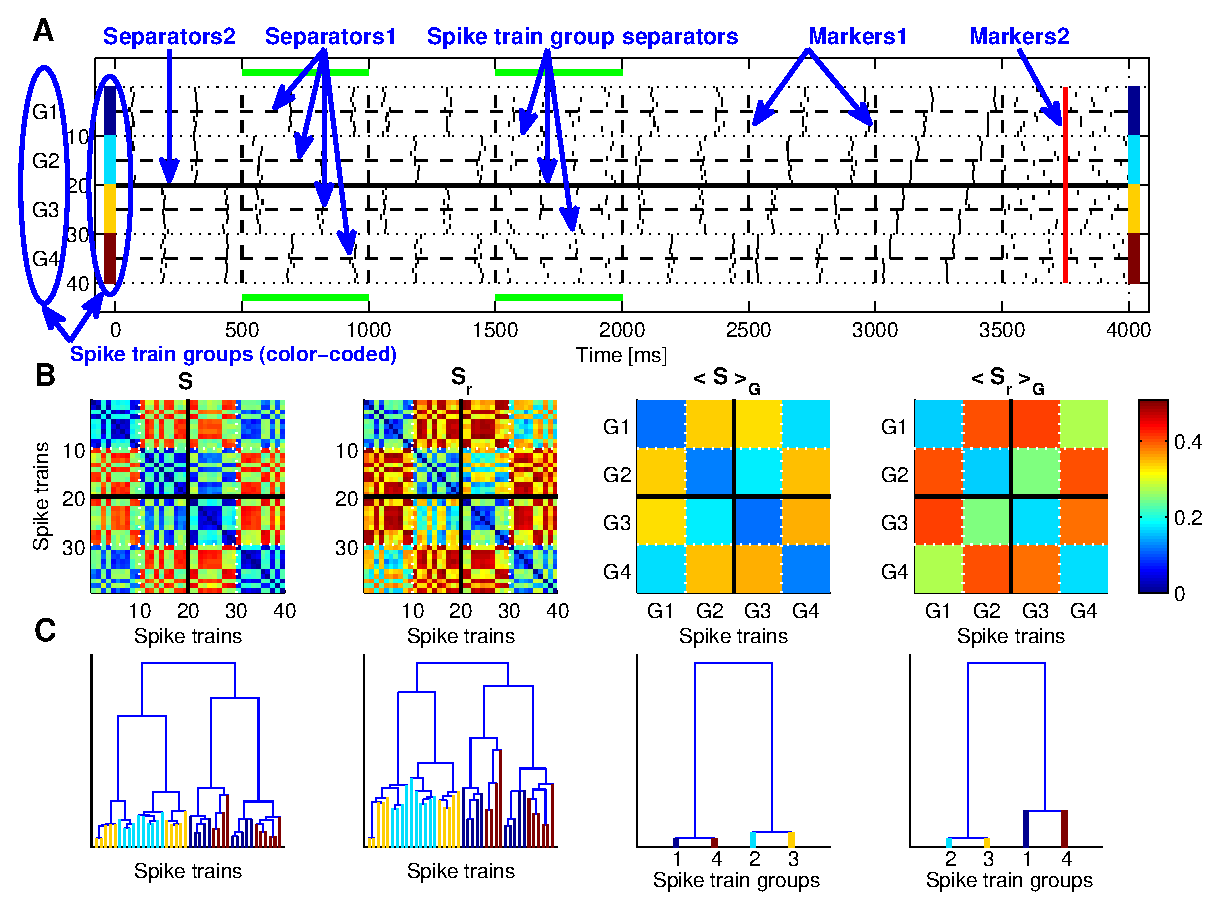
\includegraphics[width=85mm]{Fig2-Movie-Screenshot.eps}
    \caption{\abb\label{fig:Fig2-Movie-Screenshot} Annotated screenshot from a movie.   A. Artificially generated spike trains.   B. Dissimilarity matrices obtained by averaging over two separate time intervals for both the regular and the real-time SPIKE-distance as well as their averages over subgroups of spike trains (denoted by $<�>_G$).   C. Corresponding dendrograms.}
\end{figure}


\subsection{\label{ss:Spike-train-surrogates} Spike train surrogates and significance}

Daniel's Email 13.07.2011:

Regarding the use of Poisson processes to have a benchmark it will have different implications depending on the structure of your data. If the rate is almost constant then comparing to processes with the same estimated average rate is the best option. If the rate is time-dependent you may want to compare with processes which are Poissonian but mimic the same time-dependent profile of the rate. These are just alternatives that give you complementary information on the structure of the reliability.

Surrogate data with the same time dependent rate can be obtained by randomly reassigning each spike to any of the spike trains.

How can I estimate the significance of my results?
Please have a look at the program 'Spiky\_loop\_surro.m'. This is similar to 'SPIKY\_loop.m' only that you do not look at different datasets, rather you can compare the results obtained for one dataset against the results obtained for spike train surrogates generated from that dataset.

\section{\label{s:SPIKY} SPIKY}

SPIKY is a graphical user interface (GUI) for monitoring synchrony between artificially simulated or experimentally recorded neuronal spike trains. It is based on two recently proposed methods to measure spike train (dis)similarity, the ISI- and the SPIKE-distance. SPIKY is a free software package programmed by Thomas Kreuz and Nebojsa Bozanic. All source codes are written in Matlab (MathWorks Inc, MA) with the most time-consuming loops coded in MEX-files. It is not stand-alone but requires Matlab to run.

BSD licence:
Copyright (c) 2013, Thomas Kreuz, Nebojsa Bozanic
All rights reserved.

In order to get the latest information about new features and updates please like the SPIKY Facebook-Page

https://www.facebook.com/pages/SPIKY/504834062913777

This is also an opportunity to provide feedback and ask any questions you might have.

You can download a zip-package containing all the necessary files for free on http://www.fi.isc.cnr.it/users/thomas.kreuz/Source-Code/SPIKY.html.



\subsection{\label{ss:Structure} Structure of SPIKY}

First extract the zip-package (all files should be in one directory named SPIKY), then within Matlab go to this directory or add it to the path (addpath). Compile the MEX-files using SPIKY\_compile\_MEX, finally run SPIKY. 

Typically the suggested element for the next user action is marked by a bold font. The most complete initial example is entry number 5 (Clustering All) in the Data listbox. We suggest to follow this example through till the end advancing from panel to panel by pressing the highlighted button. With the same example in a second step you can start to change some parameters and see the consequences. Later, if you do not want to set all the parameters each time when you start SPIKY with a new dataset have a look at the file SPIKY\_f\_user\_interface and try to understand how for this example number 5 the spike train and the parameter values have been created. Hopefully you should then be able to do similar things with your own datasets. For quick information about the individual elements of the GUI activate the Hints-checkbox in the Options-Menu and then hover with the mouse cursor above the elements of interest and you will see short hints. An overview of all this information can be found in the file SPIKY-Elements.doc.

\subsection{\label{ss:Input} Input}

There are three possibilities:
1.	In the Selection: Data panel there is a listbox containing predefined examples. Initially these are the examples used in the paper Kreuz et al., JNeurophysiol 109, 1457 (2013) (for the complete reference see A13) but you can delete them and/or add your own data via the Matlab file 'PIKY\_f\_user\_interface'. Just make sure that the listbox entries defined in the variable listbox\_str match the examples detailed below that.
2.	You can load your own data via the Load button in the toolbar (left upper corner) or in the menu. Currently two different file formats are allowed, .mat and .txt (ASCII) files. For the mat-files SPIKY allows three different kinds of input formats:
- cell arrays (ca) with just the spike times (this is the preferred format used by SPIKY since it is most memory efficient. The two other formats will internally be converted into this format)
- regular matrices with each row being a spike train and zero padding (zp) in case the spike numbers are different.
- matrices representing time bins where each zero/one (01) indicates the absence/presence of a spike
If the spikes are stored in a Mat-file SPIKY looks for a variable called spikes, if it cannot find it you have the chance to select the variable name (or field name) which contains the spikes via some input mask which provides a hierarchical structure tree.
In the text format spike times should be written as a matrix with each row being one spike train. The package contains one example file for each format (testdata\_ca.mat, testdata\_zp.mat, testdata\_01.mat as well as testdata.txt). 
3.	You can generate your own spike trains via the Spike Train Generator. After setting some defining variables (number of spike trains, start and end time, sampling rate) you can build your spike trains by using predefined spike train patterns (such as periodic, Splay, uniform or Poisson) and/or by manually adding, shifting and deleting individual spikes or groups of spikes. For an overview of the general structure of the spike train generator please have a look at the file STG-flowchart.pdf, more detailed information can be found in the file STG-Elements.doc.


Input:
Matrix 'spikes' with two or more spike trains (if trains have different numbers of spikes, fill with zeros)
Parameter structure 'para' that describe the data (see below)
tmin:  Beginning of recording
tmax:  End of recording
dts:  Sampling interval, precision of spike times [!!! Please take care that this value is not larger than the actual sampling size, otherwise two spikes can occur at the same time instant and this can lead to problems in the algorithm !!!]
select\_measures: Vector with order of measures


\subsection{\label{ss:Output} Output}

How can I extract the spike trains and the results of the analysis (measure profiles, matrices) to the workspace
A8.  By clicking (left mouse button) on the element whose data you wish to extract. Results will be stored in variables such as SPIKY\_spikes, SPIKY\_profile\_X\_1, SPIKY\_profile\_Y\_1, SPIKY\_profile\_name\_1 as well as SPIKY\_matrix\_1 and SPIKY\_matrix\_name\_1. In addition, the results obtained during an analysis will automatically be stored in the structure SPIKY\_results which will have one field for each measure selected. 

How do I save/print figures?
A9. Press the Print to postscript button in the toolbar (left upper corner).

Output (Structure SPIKY\_results'):
SPIKY\_results.<Measure>.name:     Name of selected measures (helps to identify the order within all other variables)
SPIKY\_results.<Measure>.distance: Level of dissimilarity over all spike trains and the whole interval
                            just one value, obtained by averaging over both spike trains and time
SPIKY\_results.<Measure>.matrix:   Pairwise distance matrices, obtained by averaging over time
SPIKY\_results.<Measure>.x:        Time-values of overall dissimilarity profile
SPIKY\_results.<Measure>.y:        Overall dissimilarity profile obtained by averaging over spike train pairs

Note: For the ISI-distance the function SPIKY\_f\_pico can be used to obtain the average value as well as
x- and y-vectors for plotting (see example below):
%[overall_dissimilarity,plot_x_values,plot_y_values] = SPIKY_f_pico(SPIKY_results.isi,SPIKY_results.dissimilarity_profiles{1},para.dts,para.tmin);


\subsection{\label{ss:Figure-Layout} Figure-Layout}

To change elements (fonts, lines, etc.) in the figure simply click the right mouse button on the element you wish to change. Please use the file SPIKY\_f\_user\_interface to set the standard values for all the parameters that describe the layout of the figure (mainly the parameter structure p\_para).

How can I move subplots (spikes and profiles subplot, matrices) in the figure? How can I change their size?
Move the cursor to the respective axis (either just left or just below the subplot) and click the right mouse button. Now you can either edit all position variables by hand or change the x-position, the y-position, the width and the height individually. In case there are several matrices/dendrograms you can do this either for an individual matrix/dendrogram or for all of them at the same time.


\subsection{\label{ss:GUI-vs-loop} GUI vs. loop} 

How can I get the statistics of a certain quantity over a large number of datasets?
A14. For this purpose you can use the program SPIKY\_loop which is complementary to the graphical user interface SPIKY'. Both programs can be used to calculate time-resolved spike train distances (ISI and SPIKE) between two (or more) spike trains. However, whereas SPIKY was mainly designed to facilitate the detailed analysis of one dataset, SPIKY\_loop is meant to be used in order to compare the SPIKY\_results for many different datasets (e.g. in some kind of loop). [Note that the new program SPIKY\_loop replaces the old SPIKY\_no\_plot. The scope is the same but it adds the full functionality of SPIKY (access to time instants, selective and triggered averages as well as averages over spike train groups).]


\subsection{\label{ss:Documentation} Documentation}

SPIKY-Documentation (in extra folder SPIKY-Documentation)
SPIKY-FAQ.doc:   This file answers all the frequently asked questions regarding the graphical user interface SPIKY. 
SPIKY-Elements.doc:   This file describes all the individual elements of the graphical user interface SPIKY.
SPIKY-Files.doc:   This file containing a short description of all files contained in the SPIKY-package.
SPIKY-Flowchart.pdf:   This flowchart gives an overview of the general structure of the spike train generator.
STG-Elements.doc:   This file describes all the individual elements of the Spike Train Generator (STG).
STG-Flowchart.pdf:   This flowchart gives an overview of the general structure of the Spike Train Generator (STG).
SPIKY-Readme.doc:   This file contains a disclaimer and the BSD license.
SPIKY-no-plot.doc:   This file contains a short description of the program SPIKY\_loop which is complementary to the graphical user interface SPIKY' and meant to be used in order to compare the results for many different datasets (e.g. in some kind of loop).
Kreuz\_and\_Bozanic\_SPIKY\_Preliminary\_Draft.pdf:   This is a very preliminary draft of an upcoming article on the graphical user interface SPIKY.
SPIKY-Annotated\_Screenshot.eps:   This is an example figure taken from the 2013 paper (Fig. 8 and the supplemental movie) with some annotations detailing the various elements of a typical figure containing spike trains divided into spike train groups, dissimilarity matrices, and hierarchical cluster trees (dendrograms).
SPIKY-Screenshot.png:   Exemplary screenshot of the graphical user interface SPIKY including the use of a context menu.
STG-Screenshot.png:   Exemplary screenshot of the spike train generator (STG) including the use of a context menu.


\subsection{\label{ss:Computational-aspects} Computational aspects}

\subsection{\label{sss:Sampling} Sampling}

\subsection{\label{sss:MEX-files} MEX-files}


%
\begin{figure}
    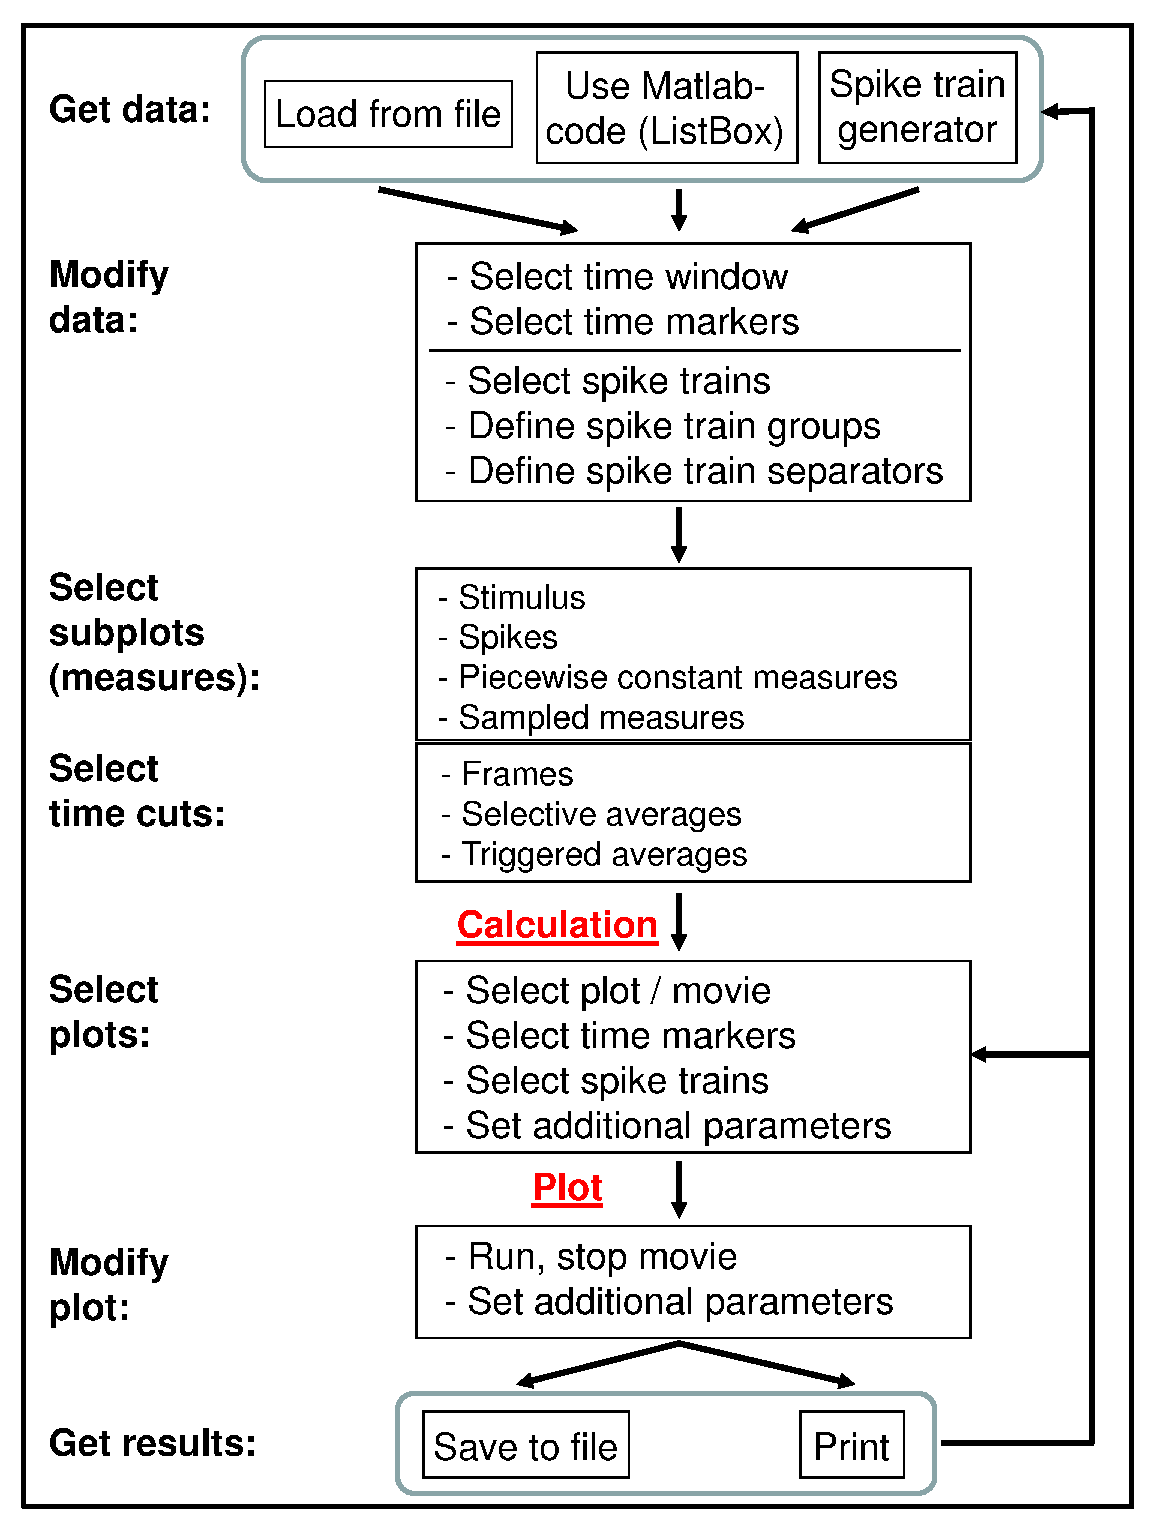
\includegraphics[width=85mm]{Fig3-SPIKY-Flowchart.eps}
    \caption{\abb\label{fig:Fig3-SPIKY-Flowchart} Annotated screenshot from a movie.   A. Artificially generated spike trains.   B. Dissimilarity matrices obtained by averaging over two separate time intervals for both the regular and the real-time SPIKE-distance as well as their averages over subgroups of spike trains (denoted by $<�>_G$).   C. Corresponding dendrograms.}
\end{figure}

XXXXX Rewrite and extend, add part on MEX-files XXXXX

The improved dissimilarity profile $S (t)$ of the SPIKE-distance is piecewise linear (with each linear interval running from one spike of the pooled spike train to the next) rather than piecewise constant as is the case for the ISI-distance.
Therefore, when the localized visualization is desired, a new value has to be calculated for each sampling point and not just once per each interval in the pooled spike train. In cases where the distance value itself is sufficient, the short computation time can be even further decreased by representing each interval by the value of its center and weighting it by its length. This is not only faster, but it actually gives the exact result, whereas the time-resolved calculation is a very good approximation only for sufficiently small sampling intervals dt (imagine the example of a rectangular function, at some point any sampled representation has to cut the right angle). The dissimilarity profiles $S_r(t)$ and $S_f (t)$ of the real-time and the future SPIKE-distances are hyperbolic and not linear but here also the exact result can be obtained by piecewise integration over all intervals of the pooled spike train.

The calculation of the SPIKE-distance consists of three steps: In a precalculation step, for each spike the distance to the nearest spike in all the other spike trains is calculated. Successively, for each time instant and each pair of spike trains, the distances of the four corner spikes are first locally weighted and then normalized. These latter steps involve
matrices of the order �number of time instants� � �number of spike train pairs�, which for very long datasets with many spike trains can lead to memory problems. The solution to these problems is to make the calculation sequential, i.e., to cut the recording interval into smaller segments, and to perform the averaging over all pairs of spike trains for
each segment separately (no additional auxiliary spikes are needed except for very huge datasets for which even the calculation of the first matrix is too memory-demanding). In the end the dissimilarity profiles for the different segments (already averaged over pairs of spike trains) are concatenated, and its temporal average yields the distance value for the whole recording interval.

The computational load scales with the number of spike trains $N$ as $N^2$. More information on the implementation as well as the Matlab source code for both the ISI- and the SPIKE-distance (including its real-time variant) can be found at www.fi.isc.cnr.it/users/thomas.kreuz/sourcecode.html.








\subsection{\label{ss:Other-Implementations} Comparison with other implementations}


XXXXXXXXXX


Python-Implementation of SPIKE-distance courtesy of Jeremy Fix:

http://jeremy.fix.free.fr/Softwares/spike.html

Python-Implementation of the pairwise ISI-distance courtesy of Michael Chary:

https://pypi.python.org/pypi/ISIpy/1.0.1

R{\v a}zvan Florian:

https://github.com/modulus-metric/spike-train-metrics

\citep{Rusu14}

The Matlab source code for calculating and visualizing the SPIKE-distance can be found under http://www.fi.isc. cnr.it/users/thomas.kreuz/sourcecode.html.


HRLAnalysis$^{TM}$ \citep{Thibeault14}




\section{\label{s:Discussion} Discussion}

\subsection{\label{ss:Summary} Summary}

\subsection{\label{ss:Limits} Limits}

\subsection{\label{ss:Outlook} Outlook}


\begin{appendix} \label{Appendix}

\end{appendix}


\vspace{1cm}

\begin{thanks}
\section{\label{s:Acknowledgement} \textbf{Acknowledgements}}
NB and TK acknowledge funding support from the European Commission through the Marie Curie Initial Training Network 'Neural Engineering Transformative Technologies (NETT)', project 289146. TK also acknowledges the Italian Ministry of Foreign Affairs regarding the activity of the Joint Italian-Israeli Laboratory on Neuroscience. 
     
We thank Emily Caporello, Daniel Chicharro, Tim Gentner, Conor Houghton, Jutta Kretzberg, Stefano Luccioli, Florian Mormann, Leon Paz, Friederice Pirschel, Alessandro Torcini, Jonathan Victor for useful discussions.

We also thank Thomas Alderson, Black Square, Mayte Bonilla Quintana, Hamid Charkhkar, Didier Desaintjan, Mario DiPoppa, Mahboubeh Etemadi, Marion Najac, Matthew Phillips, Eugenio Piasini, Robert Rein, Rodrigo Salazar, Michael Schaub, Eitan Schechtman, Matthew Williams, Yunguo Yu for advice and user feedback.
     
\end{thanks}


\bibliography{Kreuz_Bibliography}

%\bibliographystyle{plainnat}
\bibliographystyle{elsart-harv}

\end{document}
